%=========================================
% 	   Einleitung     					 =
%=========================================
\chapter{Einleitung}

\section{Aufgabenstellung}
Gemäß dem Metcalfe'schen Gesetz haben sich \textit{Social Media} zu einer der wichtigsten Informationsquellen unserer Zeit etabliert. Nutzer agieren nicht nur als Konsumenten, sondern immer mehr als Produzenten von Information. Unterstützt durch die Allgegenwärtigkeit des Internets, gelangen auf diese Weise exorbitante Mengen unstrukturierter Information in Echtzeit an die Teilnehmer des Netzwerks. Eine Selektion dieser Daten, etwa nach persönlichen Interessen, bleibt dem Nutzer meist selbst überlassen.
Als Inbegriff dieses Prinzips gilt der Mikroblogging-Dienst \textit{Twitter}. Nutzer des Dienstes können auf 140 Zeichen beschränkte Nachrichten - sogenannte \textit{Tweets} - verfassen und diese dann ungefiltert und ungeprüft veröffentlichen.\\\\
Es soll nun eine Software entwickelt werden, mit der die Selektion von Tweets automatisiert erfolgen kann. Dazu können sich Nutzer registrieren und ein Interessensprofil, bestehend aus verschiedenen Stichwörtern (\textit{Keywords}), hinterlegen. Anhand dessen wird das Gros an neuen Tweets mittels der von Twitter bereitgestellten Schnittstelle überwacht und entsprechend der darin enthaltenen Stichwörter individuell aufbereitet. Bei besonders interessanten Tweets soll der Nutzer benachrichtigt werden. Über eine Webanwendung soll es dem Nutzer darüber hinaus möglich sein, die für ihn relevanten und neuen Tweets einzusehen sowie sein Interessensprofil zu verwalten. \\\\
Die systematische Verarbeitung großer Datenmengen, im Allgemeinen unter dem Begriff \textit{Data-Mining} bekannt, stellt dabei die zentrale Herausforderung dar. Da ständig neue Daten ankommen, muss die Verarbeitung ereignisgesteuert erfolgen. Um den Datenüberschuss möglichst gering zu halten, sind schnelle Entscheidungen essentiell.
\section{TwitterStream API}
\subsection{Grundkonzept}

Die \textit{Twitter Streaming APIs} bieten eine öffentlich zugängliche Programmierschnittstelle für einen Echtzeit­Zugriff auf Daten der Social­Media­Plattform Twitter auf der Grundlage von HTTP.
\\\\
Vergleich zu REST APIs: (Twitter und andere)
Der hergebrachte Weg zu online verfügbaren Daten, sowohl für Twitter als auch bei anderen
Diensten (Facebook, GoogleEarth), erfolgt über eine REST API (Representational State Transfer).
Dabei stellt der Server einer REST­Web­Anwendung, meist auf Anfrage eines Benutzers per GET-
oder POST­Request eine entsprechende Anfrage mit den Suchparametern in der URI beim Server
des Anbieter der Daten, erhält die gewünschten Daten in der Response und gibt diese an den
Benutzer weiter. Die Anfrage vollzieht sich dabei zustandslos. Für jede Anfrage wird eine neue
TCP­Verbindung zum Anbieter aufgebaut, die (wie jede HTTP­Verbindung) nach der
Übermittlung der Daten sofort wieder durch den Anbieter­Server beendet wird. \\

\begin{figure}[!h]
    \centering
    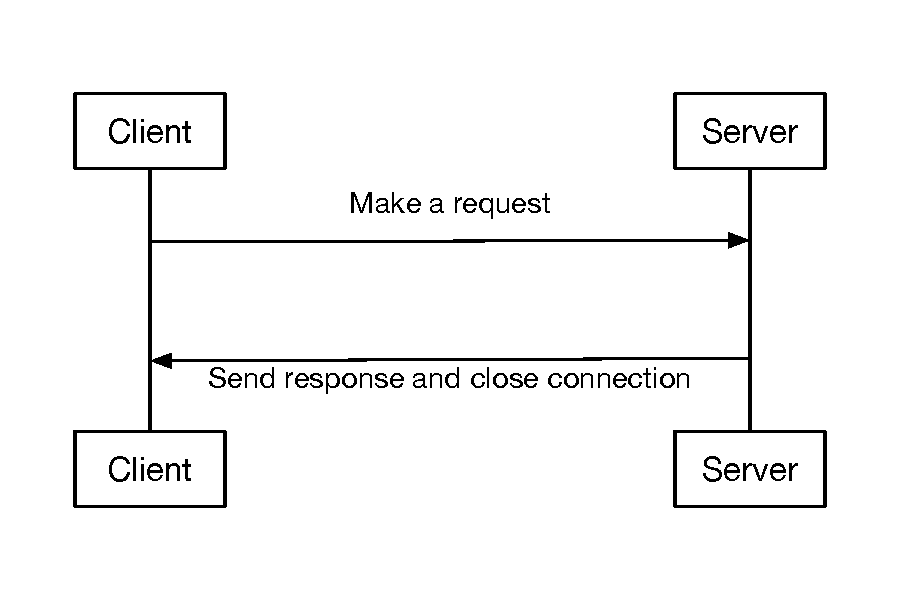
\includegraphics[width=0.85\textwidth]{Graphics/normal_rest_api}
    \caption{Grundprinzip einer REST-API}
   \label{fig:restapi}
\end{figure}
\newpage
Das Prinzip einer Streaming API beruht dagegen gerade darauf, die Verbindung zum Daten­Server
über einen längeren Zeitraum aufrecht zu erhalten. Die Verbindung wird auch hier durch einen
GET­ oder POST­Request eingeleitet, in dem gewisse Such­ oder vielmehr Filterparameter
enthalten sind. Doch der Daten­Server antwortet nicht unverzüglich mit bestimmten vorliegenden
Daten und beendet die Verbindung, sondern hält die Verbindung aufrecht und sendet
Informationen über zu den Suchparametern passende Ereignisse in Echtzeit. Auf der Client­Seite,
also beim Server der Web­Anwendung können diese Informationen dann aus dem Socket der
Verbindung gelesen werden. \\

\begin{figure}[!h]
    \centering
    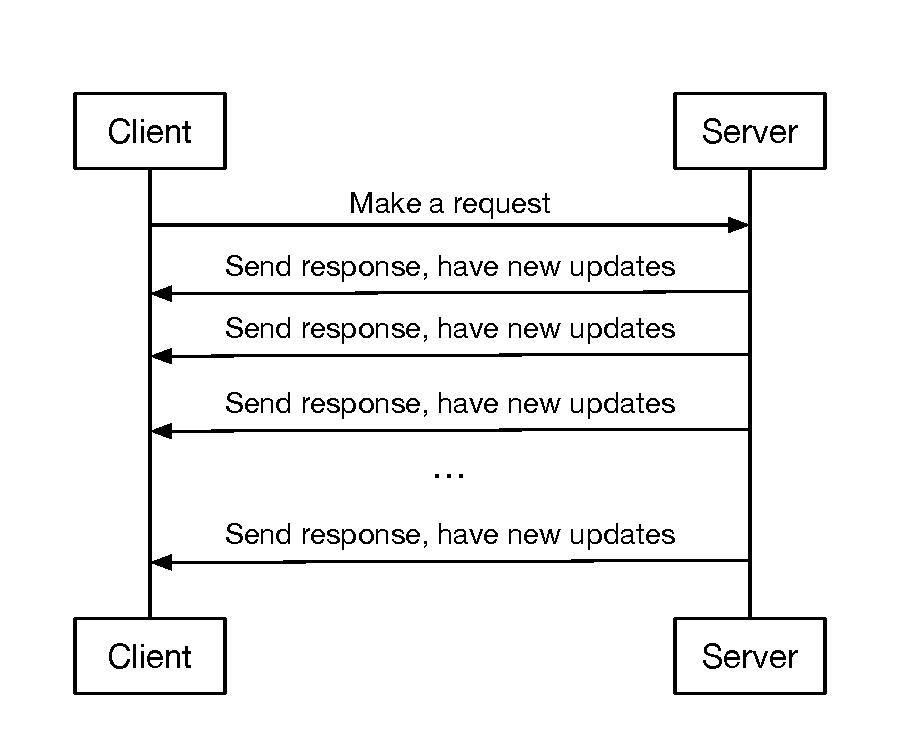
\includegraphics[width=0.85\textwidth]{Graphics/streaming_api}
    \caption{Grundprinzip einer Streaming-API}
   \label{fig:streamapi}
\end{figure}

Dieser Unterschied führt auch zu einer anderen allgemeinen Architektur eines
Anwendungsservers, der eine Streaming API verwendet. Bei Verwendung einer REST API wird
eine Anfrage meist von einem Benutzer eingeleitet und vom Anwendungsserver an die
Schnittstelle weitergereicht. Die erhaltenen Daten werden nicht langfristig gespeichert,
sondern (evtl. bearbeitet) direkt an den Benutzer geliefert. Eine permanente Verbindung kann 
hingegen nicht ständig durch den Benutzer überwacht werden und muss deshalb von der 
Serversoftware verwaltet werden. Die empfangenen Daten werden für den künftigen Zugriff 
gespeichert. Während die Serversoftware im Falle einer REST API­Anwendung also aus einer Einheit 
besteht, die sowohl für die Interaktion mit dem Nutzer als auch mit dem Daten­Server verantwortlich
ist, lassen sich bei einer typischen Streaming API zwei Teile unterscheiden. Der eigentliche
Stream wird von einem abgeschlossenen Client­Modul unabhängig vom Nutzer aufgebaut und verwaltet. Er 
erhält seine Suchparameter aus einer Datenbank, in der auch die empfangenen Daten
gespeichert werden. Der Zugang zu diesen Daten durch den Nutzer wird etwa durch ein Web-
Interface hergestellt, für das der zweite Teil als Server zuständig ist. 
\\\\
 Twitter bietet insgesamt vier Schnittstellen an. Im 
Zentrum des Projekts steht der Public Stream. Dieser wird neben anderen
Suchparametern, wie Standort oder Sprache, vor allem mit einer Liste von bis zu 400
Schlüsselwörtern initialisiert. Jeder neue Tweet, der einem oder mehreren Keyword entspricht,
wird durch den Stream geschickt. Das mögliche Datenvolumen ist also nur durch die Anzahl an
Parametern begrenzt, während alle Tweets, die den Parametern entsprechen, erfasst werden.
Allerdings ist es seitens Twitter vorgesehen, dass nur ein Public Stream pro Anwendung
existiert. Daneben werden außerdem noch User und Site Streams angeboten, die alle Tweets 
liefern, die mit einem bestimmten Twitter­Nutzer in Verbindung stehen. Der Firehose Stream
liefert schließlich bedingungs­ und ausnahmslos alle öffentlich zugänglichen Tweets. Er ist jedoch 
nicht allgemein zugänglich, sondern bedarf einer Freischaltung durch Twitter.

\section{Produktvision}

Soziale Medien haben ein gespaltenes Image. Einerseits gehören sie unumstritten zum Leben im
21. Jahrhundert. Kaum ein Ereignis wird nicht durch Twitter, Facebook und Co. dokumentiert und
kommentiert, wenn diese Plattformen nicht sogar als Katalysator wirken, der ein Ereignis erst
weltweit bekannt macht. Andererseits besteht bei der Teilnahme an dieser neuen Form der
Kommunikation auch immer die Gefahr von ihr vereinnahmt zu werden. Jede neue Form von
sozialem Medium bildet einen eigenen Mikrokosmos, dessen Regeln befolgt werden müssen, um
die angebotenen Informationen nutzen zu dürfen oder zu können. Nicht zuletzt setzt man sich
durch die Mitgliedschaft in einem sozialen Netzwerk immer auch zugleich einer höheren
Wahrscheinlichkeit aus selbst zum Diskussionsstoff zu werden. Die Alternative zur aktiven
Teilnahme an sozialen Medien, die ... einer Auswahl von Beiträgen zu einem Thema durch ein
traditionelles Medium, etwa die Tagesschau, macht wiederum gerade den Vorteil einer
ungefilterten Meinung im Internet zunichte. Es bedarf im Internet einer Möglichkeit für
Außenstehende die Kommunikation in sozialen Netzwerken nach eigenem Ermessen zu
beobachten. Durch Anwendungen nach dem REST­Prinzip sind nur gezielte Zugriffe auf die
Vergangenheit möglich. Es fehlt jedoch eine Möglichkeit, um auf die aktuelle Kommunikation
zugreifen zu können.\\
Das Ziel dieses Projekts ist es diese Lücke zu schließen. Es wird eine Webanwendung erstellt, in
der sich Benutzer mit einem möglichst geringen Verwaltungsüberbau anmelden und beliebige
Schlüsselwörter anlegen, die ihren Interessen entsprechen. Diese werden zur Schlüsselwortliste
eines Public Streams hinzugefügt, so dass sämtliche Tweets, die sie enthalten, während der
Abwesenheit des Nutzers erfasst und in einer Datenbank gespeichert werden. Dem Nutzer stehen
die seinen Schlüsselwörtern entsprechenden Tweets in einer Übersicht zur Verfügung, die er selbst
noch einmal nach beliebigen Schlüsselwörtern und anderen Parametern filtern kann. Um den
Vorteil des Echtzeitzugriffs auf aktuelle Ereignisse durch einen Stream auszunutzen, soll dem
Benutzer außerdem die Möglichkeit gegeben werden, seine Email­Adresse zu hinterlassen, so dass
er automatisch über neu eingetroffene Tweets unterrichtet wird.


